\documentclass{beamer}
\mode<presentation>
\usepackage{amsmath}
\usepackage{amssymb}
%\usepackage{advdate}
\usepackage{adjustbox}
\usepackage{subcaption}
\usepackage{enumitem}
\usepackage{multicol}
\usepackage{mathtools}
\usepackage{listings}
\usepackage{url}
\usepackage{tikz}
\usepackage{tcolorbox}
\usetikzlibrary{matrix}\def\UrlBreaks{\do\/\do-}
\usetheme{metropolis}
%\usecolortheme{lily}
\setbeamertemplate{footline}
{
  \leavevmode%
  \hbox{%
    \begin{beamercolorbox}[wd=\paperwidth,ht=2.25ex,dp=1ex,right]{author in head/foot}%
      \insertframenumber{} / \inserttotalframenumber\hspace*{2ex} 
    \end{beamercolorbox}}%
    \vskip0pt%
  }
  \setbeamertemplate{navigation symbols}{}

  \providecommand{\nCr}[2]{\,^{#1}C_{#2}} % nCr
  \providecommand{\nPr}[2]{\,^{#1}P_{#2}} % nPr
  \providecommand{\mbf}{\mathbf}
  \providecommand{\pr}[1]{\ensuremath{\Pr\left(#1\right)}}
  \providecommand{\qfunc}[1]{\ensuremath{Q\left(#1\right)}}
  \providecommand{\sbrak}[1]{\ensuremath{{}\left[#1\right]}}
  \providecommand{\lsbrak}[1]{\ensuremath{{}\left[#1\right.}}
  \providecommand{\rsbrak}[1]{\ensuremath{{}\left.#1\right]}}
  \providecommand{\brak}[1]{\ensuremath{\left(#1\right)}}
  \providecommand{\lbrak}[1]{\ensuremath{\left(#1\right.}}
  \providecommand{\rbrak}[1]{\ensuremath{\left.#1\right)}}
  \providecommand{\cbrak}[1]{\ensuremath{\left\{#1\right\}}}
  \providecommand{\lcbrak}[1]{\ensuremath{\left\{#1\right.}}
  \providecommand{\rcbrak}[1]{\ensuremath{\left.#1\right\}}}
  \theoremstyle{remark}
  \newtheorem{rem}{Remark}
  \newcommand{\sgn}{\mathop{\mathrm{sgn}}}
  \providecommand{\abs}[1]{\left\vert#1\right\vert}
  \providecommand{\res}[1]{\Res\displaylimits_{#1}} 
  \providecommand{\norm}[1]{\lVert#1\rVert}
  \providecommand{\mtx}[1]{\mathbf{#1}}
  \providecommand{\mean}[1]{E\left[ #1 \right]}
  \providecommand{\fourier}{\overset{\mathcal{F}}{ \rightleftharpoons}}
  %\providecommand{\hilbert}{\overset{\mathcal{H}}{ \rightleftharpoons}}
  \providecommand{\system}{\overset{\mathcal{H}}{ \longleftrightarrow}}
  %\newcommand{\solution}[2]{\textbf{Solution:}{#1}}
  %\newcommand{\solution}{\noindent \textbf{Solution: }}
  \providecommand{\dec}[2]{\ensuremath{\overset{#1}{\underset{#2}{\gtrless}}}}
  \newcommand{\myvec}[1]{\ensuremath{\begin{pmatrix}#1\end{pmatrix}}}
    \let\vec\mathbf

    \lstset{
      %language=C,
      frame=single, 
      breaklines=true,
      columns=fullflexible
    }

    \numberwithin{equation}{section}

    \title{NCERT Presentation}
    \author{Arjun Pavanje,\\ EE24BTECH11005,\\IIT Hyderabad.\\}

    \date{\today} 
    \begin{document}

    \begin{frame}
      \titlepage
    \end{frame}

    \section*{Table of Contents}
    \begin{frame}
      \tableofcontents
    \end{frame}
    \section{Problem}
    \begin{frame}
      \frametitle{Problem Statement}

      In a class test, the sum of Shefali's marks in Mathematics and English is $30$. Had she got $2$ marks more in Mathematics and $3$ marks less in English, the product of their marks would have been $210$. Find her marks in the two subjects. \newline

    \end{frame}
    \section{Solution}
    \subsection{solution}
    \begin{frame}
      \frametitle{Solution}
      In a class test, the sum of Shefali's marks in Mathematics and English is $30$. Had she got $2$ marks more in Mathematics and $3$ marks less in English, the product of their marks would have been $210$. Find her marks in the two subjects. \newline
      Let $x, y$ be the marks obtained in Mathematics and English respectively. 
      \begin{align}
        x + y = 30\\
        \brak{x+2}\brak{y-3} = 210
      \end{align}
      On combining the above two equations we get,
      \begin{align}
        x^2 - 25x + 156
      \end{align} 
    \end{frame}
    \subsection{Newton-Ralphson Method}
    \begin{frame}
      \frametitle{Newton-Ralphson Method}
      Start with an initial guess $x_0$, and then run the following logical loop,
      \begin{align}
        x_{n+1} = x_n - \frac{f\brak{x_n}}{f^{\prime}\brak{x_n}} 
      \end{align}
      where,
      \begin{align}
        f\brak{x} = x^2 - 25x + 156\\
        f^{\prime}\brak{x} = 2x - 25
      \end{align}
      The update equation will be
      \begin{align}
        x_{n+1} = x_n - \frac{{x_n}^2 - 25x_n + 156}{2x_n - 25}\\
      \end{align}
    \end{frame}
    \begin{frame}
      \frametitle{Newton-Ralphson Method}
      The output of a program written to find roots is shown below:
      \begin{align}
        x = 12.000000000000014 \\
        x = 12.999999999999964
      \end{align}    
    \end{frame}
    \subsection{Eigenvalue Solution}
    \begin{frame}
      \frametitle{Companion Matrix}
      For a polynomial equation of form $x_n+c_{n-1}x^{n-1}+\dots+c_2x^2+c_1x+c_0 = 0$ we construct a matrix called companion matrix of form
      {\small
      \begin{align}
        \myvec{
          0 & 0 & \cdots & 0 & -c_0\\
          1 & 0 & \cdots & 0 & -c_1\\
          0 & 1 & \cdots & 0 & -c_2\\
          \vdots & \vdots & \ddots & \vdots & \vdots\\
          0 & 0 & \cdots & 1 & -c_{n-1}\\
        }
      \end{align}}
      The eigenvalues of the companion matrix are the roots of the polynomial equation.  For the given question, the companion matrix comes out to be,
      {\small
      \begin{align}
        \myvec{0 & -156 \\ 1 & 25}
      \end{align}
      }
    \end{frame}
    \begin{frame}
      \frametitle{Schur Decomposition}
      Using QR decomposition algorithm, we will now solve for the eigenvalues of the above companion matrix. \newline \newline Basic principle behind iterative QR decomposition is similar matrices.
      Two square matrices $A$ and $B$ of size $n \times n$ are said to be $similar$ if there exists an invertible matrix $P$ such that:
      \begin{align}
        B = P^{-1} A P.
      \end{align}
      Similar matrices turn out to have the same eigenvalues. This can be easily proved,

      Given that $A$, $B$ are similar matrices, and $P$ is an invertible matrix such that $B=P^{-1}AP$
      By definition of eigenvalues,
    \end{frame}
    \begin{frame}
      \frametitle{Schur Decomposition}
      {\small
      \begin{align}
        \det(B-\lambda I)&=\det(P^{-1}AP -\lambda I)\\
        &=\det(P^{-1}AP -\lambda P^{-1}P)\\
        &=\det(P^{-1})\det(A-\lambda I)\det(P)\\
        &=\det(P^{-1}P)\det(A- \lambda I)\\
        &=\det(A-\lambda I)
      \end{align}
      }
      Basic idea is to use similarity transforms repeatedly on the matrix till it converges to an Upper-Triangular Matrix. The eigenvalues will just be the principal diagonal elements of the matrix.
    \end{frame}
    \begin{frame}[fragile]
      \frametitle{Steps}
      Steps to perform QR decomposition and accelerate its convergence,\newline
      1. Convert to Upper Hessenberg form via Householder Reflections \newline
      2. Performing QR decomposition via Givens Rotations with shifts \newline
      3. Read off diagonal elements
    \end{frame}
    \begin{frame}
      \frametitle{Householder Reflections}
      A square matrix A of order $n \times n$ is said to be in upper Hessenberg form if all the entries below the first subdiagonal are zero.
      For example:
      {\small
      \begin{align}
        H = \begin{bmatrix}
          \times & \times & \times & \times \\
          \times & \times & \times & \times \\
          0 & \times & \times & \times \\
          0 & 0 & \times & \times
        \end{bmatrix}.
      \end{align}
      }
      Applying QR decomposition to reach Schur-form to the matrix after it is in Upper Hessenberg form greatly accelerates rate of convergence.\\
      Householder transformations are used to reduce a general matrix $A$ to Upper Hessenberg form. A Householder reflector is an orthogonal matrix defined as:
      \begin{align}
        P = I - 2\textbf{uu}^{\top} \\
      \end{align}
    \end{frame}
    \begin{frame}
      \frametitle{Householder Reflections}
      where $\|\textbf{u}\|=1$\\    
      Vector $\textbf{u}$ must be carefully chosen such that the resultant matrix $P$ obtained from it must zero out all elements below the first subdiagonal for that particular column while maintaining similarity to preserve eigenvalues.\newline
      For a given column vector $x \in \mathbb{R}^n$, the vector $u$ is chosen as:
      \begin{align}
        \mathbf{u} = \frac{\mathbf{x} - \|\mathbf{x}\| \rho \mathbf{e_1}}{\|\mathbf{x} - \|\mathbf{x}\| \rho \mathbf{e_1}\|}
      \end{align}
    where $\rho$ is something we have a degree of freedom in choosing as long as $\abs{\rho}=1$
    \end{frame}
    \begin{frame}
      \frametitle{Householder Reflections}

      Usually, $\rho=-sign(x_1)$, but here for ease of calculation $\rho= -e^{j\phi}$ where $x_1=|x_1| e^{j\phi}$\\
      Visualizing the process,
      \begin{align}
        \begin{bmatrix}
          \times & \times & \times & \times \\
          \times & \times & \times & \times \\
          \times & \times & \times & \times \\
          \times & \times & \times & \times
        \end{bmatrix}
        \xrightarrow{P_1}
        \begin{bmatrix}
          \times & \times & \times & \times \\
          \times & \times & \times & \times \\
          0 & \times & \times & \times \\
          0 & \times & \times & \times
        \end{bmatrix}
        \xrightarrow{P_2}
        \begin{bmatrix}
          \times & \times & \times & \times \\
          \times & \times & \times & \times \\
          0 & \times & \times & \times \\
          0 & 0 & \times & \times
        \end{bmatrix}.
      \end{align}      \end{frame}
      \begin{frame}
        \frametitle{Givens Rotations}


        A Givens rotation matrix $(G(i,j,\theta)$ zeroes out the element $a_{ij}$ by rotating in the $(i,j)$-plane. It is defined as:
        {\small
        \begin{align*}
          G(i, j, \theta) = \begin{bmatrix}
            1 & \cdots & 0 & \cdots & 0 & \cdots & 0 \\
            \vdots & \ddots & \vdots & \ddots & \vdots & \ddots & \vdots \\
            0 & \cdots & c & \cdots & s & \cdots & 0 \\
            \vdots & \ddots & \vdots & \ddots & \vdots & \ddots & \vdots \\
            0 & \cdots & -\overline{s} & \cdots & \overline{c} & \cdots & 0 \\
            \vdots & \ddots & \vdots & \ddots & \vdots & \ddots & \vdots \\
            0 & \cdots & 0 & \cdots & 0 & \cdots & 1
          \end{bmatrix}
        \end{align*}
        }
        where $\cos\theta$ and $\sin\theta$ are chosen such that the target element is eliminated.\\
      To choose the values of $c$ and $s$ for the Givens rotation in QR decomposition, let $a_j$ be the element we wish to null out (i.e. make 0).         \end{frame}
      \begin{frame}
        \frametitle{Givens Rotations}
        Pick an arbitrary non-zero pivot element $a_i$ (on a different row). Usually, if we wish to null a particular sub-diagonal element, we pick the principal diagonal element above it as a pivot.
        \begin{align*}
          c = \frac{\overline{a_{i}}}{\sqrt{a_{i}^2 + a_{j}^2}}, \quad s = \frac{-\overline{a_{j}}}{\sqrt{a_{i}^2 + a_{j}^2}}
        \end{align*}
        Givens rotation essentially rotates the two rows that $a_i$ and $a_j$ are on such that $a_j = 0$ after rotation, other rows remain unaffected. 

      \end{frame}
      \begin{frame}
        \frametitle{Givens Rotations}
        Visualizing the process,
        {\small
        \begin{align}
          \begin{bmatrix}
            \times & \times & \times & \times \\
            \times & \times & \times & \times \\
            0 & \times & \times & \times \\
            0 & 0 & \times & \times
          \end{bmatrix}
          \xrightarrow{G(3,2,\theta_1)}
          \begin{bmatrix}
            \times & \times & \times & \times \\
            \times & \times & \times & \times \\
            0 & 0 & \times & \times \\
            0 & 0 & \times & \times
          \end{bmatrix}
          \xrightarrow{G(4,3,\theta_2)}
          \begin{bmatrix}
            \times & \times & \times & \times \\
            \times & \times & \times & \times \\
            0 & 0 & \times & \times \\
            0 & 0 & 0 & \times
          \end{bmatrix}.
        \end{align}
        }
        After all Givens rotations, the resulting matrix is upper triangular:
        {\small
        \begin{align}
          R = \begin{bmatrix}
            \times & \times & \times & \times \\
            0 & \times & \times & \times \\
            0 & 0 & \times & \times \\
            0 & 0 & 0 & \times
          \end{bmatrix}.
        \end{align}
        }
      \end{frame}
      \begin{frame}
        \frametitle{Givens Rotations}
        The sequence of Givens rotations $G_1, G_2, \dots, G_m$ satisfies:
        \begin{align}
          G_m \cdots G_2 G_1 A = R,
        \end{align}
        where \(R\) is upper triangular. The QR decomposition is obtained by combining the transposes of the Givens rotations into \(Q\):
        \begin{align}
          A = Q R, \quad Q = G_1^{\top} G_2^{\top} \cdots G_m^{\top}.
        \end{align}
        \begin{align}
          A_{k+1}&= R_k Q_k\\
          &=(G_n \dots G_2 G_1)A_k(G_1^{\top}G_2^{\top}\dots G_n^{\top})\\
          &= (G_n \dots G_2 G_1)A_k(G_n \dots G_2 G_1)^{\top}
        \end{align}
        Iteratively repeating this process causes the matrix to converge to upper triangular.
      \end{frame}
      \begin{frame}
        \frametitle{Result}
Running the eigenvalue code for our companion matrix we get,
Eigenvalues:
(11.999964 + 0.000000i) 
(13.000036 + 0.000000i)
      \end{frame}
\subsection{Graph}
      \begin{frame}[fragile]
        \frametitle{Graph}
        \begin{figure}[h!]
          \centering
          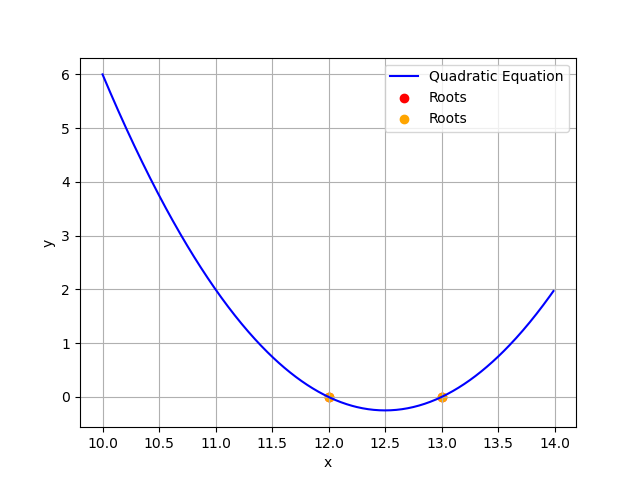
\includegraphics[width=1\columnwidth]{figs/fig.png}
          \label{stemplot}
        \end{figure}
      \end{frame}
    \end{document}
